\section{Ungleichungen}

Autor: Marc Mittner

\noindent "Uberarbeitung: Christian Rutsch

\subsection{Definition}
Eine Ungleichung stellt eine Ordnung zweier mathematischer Objekte dar. Ungleichungen werden bez"uglich der Anzahl der Variablen und der Potenz, in der die Variablen auftreten, unterschieden. Dabei variiert je nach Typ der Ungleichung das L"osungsverfahren.

\subsection{"Aquivalenzumformung von Ungleichungen}
Zur Umformung von Ungleichungen sind folgende Operationen zul"assig:
\begin{itemize}
\item{Addition einer Zahl $a \in \mathbb{R}$ auf beiden Seiten.}
\item{Subtraktion einer Zahl $a \in \mathbb{R}$ auf beiden Seiten.}
\item{Multiplikation/Division mit einer Zahl $a \in \mathbb{R}, a > 0$ auf beiden Seiten.}
\item{Multiplikation/Division mit einer Zahl $a \in \mathbb{R}, a < 0 $ auf beiden Seiten. Dabei ist zu beachten, dass das Ordnungszeichen umgedreht wird!}
\item{Bei Ziehen der Quadratwurzel muss darauf geachtet werden, dass die Ungleichung in zwei Teile zerf"allt:
\begin{align*}
x^2 < a^2 &\Leftrightarrow \\
-a < x < a &\Leftrightarrow \\
 |x| < a &
\end{align*}
(siehe Beispiel bei quadratischen Ungleichungen).}
\end{itemize}
"Anderung der Ordnungszeichen bei Multiplikation/Division mit einer Zahl $ a < 0 $:
\begin{itemize}
\item $ < $ wird zu $ > $, aus $ > $ wird $ < $
\item $ \leq $ wird zu $ \geq $, aus $ \geq $ wird $ \leq $
\item Die Zeichen "`$ = $"' und "`$ \neq $"' bleiben erhalten.
\end{itemize}
Nicht generell erlaubt sind folgende Umformungen:
\begin{itemize}
\item beidseitige Multiplikation mit 0
\item beidseitige Division durch 0
\item beidseitiges Quadrieren 
\end{itemize}


\subsection{Lineare Ungleichungen}
Eine lineare Ungleichung ist eine Ungleichung, in der die Variable nur in der ersten Potenz enthalten ist. Jede lineare Ungleichung kann in eine dieser drei Formen gebracht werden:
\[ax + b > c\quad \text{ oder }\quad
ax + b \geq c\quad \text{ oder }\quad
ax + b \neq c \]


\noindent Zur L"osung einer linearen Ungleichung wird die Variable durch Umformen isoliert:

Beispiel:
\begin{align*}
3 - 4x - 13 + 2x - 3x + 12 &\leq 5 && \text{Zusammenfassen}\\
-5 x + 2 & \leq 5 && |\ -2 \\
-5x &\leq 3 &&|\ \div (-5) \\
 x &\geq - \frac{3}{5}
\end{align*}

Graphische Darstellung des L"osungsbereichs:
\begin{center}
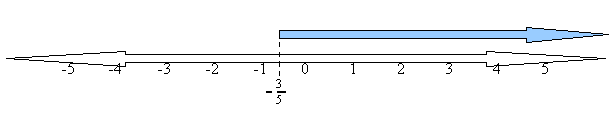
\includegraphics[width=0.8\textwidth]{img/ungleichungen/LBer1.png}
\end{center}

Allgemein:
\begin{align*}
ax + b &\leq c &&| -b\\
ax &\leq c - b &&|\div a ~(a > 0) \\
x &\leq \frac {c - b} a
\end{align*}


\subsection{Quadratische Ungleichungen}

Bei quadratischen Ungleichungen k"onnen Variablen auch in der zweiten Potenz
auftreten. Jede quadratische Ungleichung kann in eine der Formen 
\[x^2 + px + q > r 
\quad \text{oder} \quad
x^2 + px + q \geq r 
\quad \text{oder} \quad
x^2 + px + q \neq r \]
zusammengefasst werden.

\noindent Zur L"osung wird das Verfahren der quadratischen Erg"anzung verwendet.
Bei diesem Verfahren wird zur normierten Form der quadratischen Ungleichung 
\[x^2 + px + q > r\] der Teil $x^2 + px$ zu einer binomischen Formel erweitert.

Allgemein:
\begin{align*}
x^2 + px + q &< r &&|-q
\intertext{Quadratische Erg"anzung:}
x^2 + px &< r - q &&|+ \left(\frac{1}{2} p \right)^2\\
x^2 + px + \left(\frac{1}{2} p \right)^2 &< r - q + \left(\frac{1}{2} p \right)^2 && \text{Binom} \\
\left(x + \frac{1}{2} p \right)^2 &< r - q + \left(\frac{1}{2} p \right)^2\\
|x + \frac{1}{2} p| &< \sqrt{ r - q + \left(\frac{1}{2} p \right)^2}
\end{align*}

Daraus folgen die beiden L"osungen:
\begin{align*}
x_1 &< \phantom{-}\sqrt{r  - q + \left(\frac{1}{2} p \right)^2} - \frac{1}{2} p\\
x_2 &> -\sqrt{r - q + \left(\frac{1}{2} p \right)^2} - \frac{1}{2} p
\end{align*}
Somit erh"alt man die p-q-Formel f"ur quadratische Gleichungen in normierter Form ($r = 0$):
\[x_{1,2} = - \frac p 2 \pm \sqrt{ \left( \frac p 2 \right)^2 - q}\]

\paragraph*{Beispiel:}
\begin{align*}
5x^2 + 12 - 12x - 3x^2 &\geq 26 &&\text{Zusammenfassen}\\
2x^2 - 12x + 12 &\geq 26 &&\text{Normieren} \\
x^2 - 6x + 6 &\geq 13 &&|-6 \\
\intertext{Quadratische Erg"anzung:}
x^2 - 6x &\geq 7 &&|+9\\
x^2 - 6x + 9 &\geq 16 &&\text{2. binom. Formel}\\
(x - 3)^2 &\geq 16
\intertext{Die Ungleichung zerf"allt in zwei Teile:}
|x - 3| &\geq 4 
\intertext{1. Fall:}
x_1 - 3 &\geq 4\\
x_1 &\geq 7
\intertext{2. Fall:}
-x_2 + 3 &\geq 4\\
x_2 &\leq -1
\end{align*}

Graphische Darstellung des L"osungsbereichs:
\begin{center}
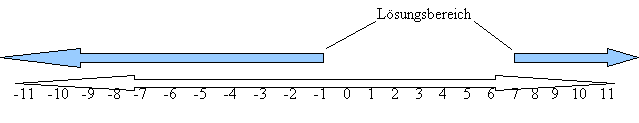
\includegraphics[width=0.8\textwidth]{img/ungleichungen/LBer2.png}
\end{center}

\subsection{Ungleichungen h"oherer Ordnung}

Zum L"osen von Ungleichungen h"oherer Ordnung eignet sich wegen der Komplexit"at der Gleichungen meist nur die Darstellung der Gleichung als Produkt in der Form: 
\[(x - a_1) \cdot (x - a_2) \cdot \ldots \cdot (x - a_n) > 0 \]
Die analytische Berechnung der Nullstellen ist aber nicht immer m"oglich. Lediglich bei Ungleichungen der Ordnung drei ist diese Faktorisierung noch praktikabel.

\subsection{Bruchungleichungen}

Bei Bruchungleichungen ist darauf zu achten, dass zuerst der Definitionsbereich festgestellt werden muss, da eine Division durch Null nicht zul"assig ist. Dazu werden alle Belegungen der Variablen, die eine solche Division verursachen w"urden, aus dem Definitionsbereich entnommen.

\subsubsection{L"osen von Bruchungleichungen}

Zum L"osen von Bruchungleichungen benutzt man folgende Vorgehensweise:
\begin{enumerate}
\item Multiplikation beider Seiten mit dem Hauptnenner
\item Ausmultiplizieren
\item L"osen der entstehenden (quadratischen) Ungleichung
\end{enumerate}

\subsubsection{Beispiel}

\begin{align*}
\frac{(3x - 2)} {(x + 2)} + \frac{(2 + 5x)} {(x^2 - 4)} &\leq \frac{(x + 3)} {(x - 2)}\\
\intertext{Definitionsbereich $ D = \mathbb{R} \setminus \lbrace -2 , +2 \rbrace $}
\intertext{Multiplikation mit dem Hauptnenner $ (x + 2)(x - 2) = (x^2 - 4) $:}
\frac{(3x - 2)} {(x + 2)} \cdot (x^2 - 4) + \frac {(2 + 5x)} {(x^2 - 4)} \cdot (x^2 - 4) &\leq \frac{(x + 3)} {(x - 2)} \cdot (x^2 - 4)\\
(3x - 2)(x - 2) + 2 + 5x &\leq (x + 3)(x + 2)\\
\intertext{Ausmultiplizieren:}
3x^2 - 8x + 4 + 2 + 5x &\leq x^2 + 5x + 6\\
\intertext{L"osen der entstandenen quadratischen Gleichung:}
 2x^2 - 8x &\leq 0 \\
 x^2 - 4x) &\leq 0 \\
 x^2 - 4 x + 4 &\leq 4 \\
 |x - 2| &\leq 2 \\
x &\leq 4 \\
 x &\geq 0
\end{align*}
L"osung für die Ungleichung sind somit alle $ x $ mit $ 0 \leq x \leq 4 $ außer $ x = 2 $, da diese Belegung nicht im Definitionsbereich liegt und somit auch nicht im L"osungsbereich liegen kann.
$L = \lbrace x \in \mathbb{R}\ |\ 0 \leq x \leq 4 ,x \neq 2\rbrace $

Graphische Darstellung des L"osungsbereichs:
\begin{center}
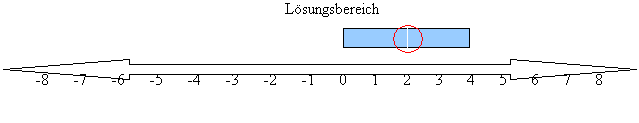
\includegraphics[width=0.8\textwidth]{img/ungleichungen/LBer3.png}
\end{center}

\subsection{Ungleichungen mit mehreren Variablen}

Ungleichungen mit mehreren Variablen haben statt einem eindimensinalen einen mehrdimensinalen L"osungsbereich. Die Dimension nimmt mit der Anzahl der Variablen zu. So hat ein Ungleichungssystem mit zwei Variablen eine L"osung im $ \mathbb{R}^2 $ (also in einer Ebene) und Ungleichungssysteme mit $n$ Variablen haben eine L"osung im $\mathbb{R}^n$.

\subsubsection{Beispiel: Ungleichung mit 2 Variablen}

\begin{align*}
2x^2 + 3 - y - 2 &> 2 \\
2 - \frac{1}{2} x &< \frac{1}{2} y + 2
\end{align*}

Zum L"osen des Ungleichungssystems wird zuerst eine Variable isoliert.
\begin{align*}
y &< 2x^2 - 1 \\
y &> -x
\end{align*}

Dadurch ergibt sich nun:
\[ 2x^2 - 1 > y > -x \]

%\newpage
Graphische Darstellung des L"osungsbereichs:
\begin{center}
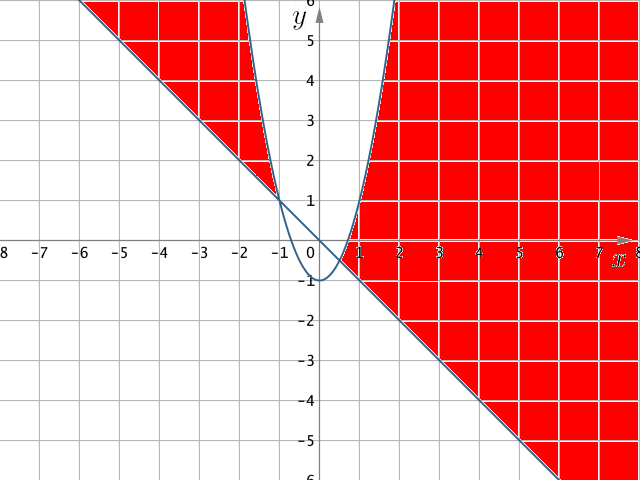
\includegraphics[width=0.5\textwidth]{img/ungleichungen/UGlsystmit2.png}
\end{center}

Der markierte Bereich stellt den L"osungsbereich dar. \\
Die Punkte auf den Funktionen selbst sind nicht im L"osungsbereich enthalten. \\
F"ur den Bereich $ -1 \leq x \leq \frac{1}{2} $ existiert keine L"osung. \\
F"ur alle anderen Werte von $x$ sind alle Punkte, f"ur die die Bedingung
\[ 2x^2 - 1 > y > -x \] erf"ullt ist, in der L"osungsmenge enthalten.

\subsection{Quellen}
\small
\begin{itemize}
\item{\url{http://ilias.tfh-wildau.de/~laborwww/downloads/Kap2_komplett.pdf}}
\item{Wikipedia: L"osen von Ungleichungen}
\item{\url{ftp://ftp.fernuni-hagen.de/pub/fachb/mathe/alggeo/schulte/1011C3.pdf} \linebreak (nicht mehr verfügbar)}
\end{itemize}
\normalsize

\subsection{Aufgaben}

\subsubsection{Ungleichungen mit einer Variablen}
L"osen Sie folgende Ungleichungssysteme analytisch:
\begin{enumerate}\abovedisplayskip-1em
\item{ \begin{align*}(x+1)(x-1) &\leq 0\\ \sqrt{x} &\geq 1\end{align*}}
\item{ \begin{align*}\sqrt{\frac{1}{2}x^3 +2x^2 +\frac{21}{8}x + \frac{9}{8}} < \sqrt{\frac{1}{2}x^2 + \frac{3}{2}x+\frac{9}{8}} \end{align*} }
\item{ \begin{align*}\frac{1}{2}x^2-1 &> 0\end{align*}}
\item{ \begin{align*}x^3 +3x^2 -4 &> 0\end{align*}}
\item{ \begin{align*}x^3 +3x^2 +3x +1 &< 0\end{align*}}
\item{ \begin{align*}x^6 -6x^5 + 15x^4 -20x^3 +15x^2 -6x +1 &\leq 0\end{align*}}
\item{ \begin{align*}\frac{1}{2}x^2 -8 &> 0\\-3(x-1)^2 +12 &> 0\end{align*}}
\item{ \begin{align*}(x^2-2)(x+1) &\geq 0\end{align*}}
\item{\abovedisplayskip1em Geben Sie die L"osungsmenge des Ungleichungssystems in Abh"angigkeit von \textit{a} an.\begin{align*}ax^2 &> 0\\ \frac{1}{2}x + 1 &> 0\end{align*}}
\item{\abovedisplayskip1em Geben Sie die L"osungsmenge des Ungleichungssystems in Abh"angigkeit von \textit{a} an. \begin{align*}x^2 + a &> 0\\ \frac{1}{2}x +1 &> 0\end{align*}}
\item{\abovedisplayskip1em Geben Sie die L"osungsmenge des Ungleichungssystems in Abh"angigkeit von \textit{a} an. \begin{align*}-x^2 +a &< 0\\ x+a &< 0\end{align*}}
\item{\abovedisplayskip1em Geben Sie die L"osungsmenge des Ungleichungssystems in Abh"angigkeit von \textit{a} an. \begin{align*}4x^2-2ax+\frac{1}{4}a^2 &\geq 0\end{align*}}
\item{ \begin{align*}x^3+x^2-2x &\geq 2\end{align*}}
\item{ \begin{align*}(x-1)^2 -4 &< 0\\ -(x+1)^2 +4 &> 0\end{align*}}
\item{ \begin{align*}\sqrt{(x-1)} &\geq 0\\ -\frac{1}{4x}+4 &< 0\end{align*}}
\item{ \begin{align*}x^4-16 &\leq 0\\ x^3 +1 &\geq 0\end{align*}}
\end{enumerate}

\subsubsection{Ungleichungen mit mehreren Variablen}
L"osen Sie folgende Ungleichungssysteme graphisch:
\begin{enumerate}\abovedisplayskip-1em
\item{ \begin{align*}x^2 +y^2 &< 25\\ \frac{1}{2}x +\frac{5}{2} &> y\\ -x-5 &< y\end{align*}}
\item{ \begin{align*}-x^2 +5 &< y\\ x(x-3)^2 &> y\\ -x-2 &> y\end{align*}}
\item{ \begin{align*}3x^2-3x-10 &< -4 +y\\ y &\leq \frac{1}{2}\end{align*}}
\item{ \begin{align*}y &< \frac{2x^2+3x+4}{-x^4-2x^3-x^2+4x+(2x+x^2)^2}\\ -\frac{1}{x} &< y\\ -(\frac{1}{\sqrt{2}}x)^2 &< y - \frac{1}{2}x^2 + \frac{1}{2}x +2\\ y+x-2<0\end{align*}}
\item{ \begin{align*}\frac{1}{2}x^2 - 3x &\leq y\\ y &\leq -x\\ 17x^3 - \frac{1}{2} &= y\end{align*}}
\item{ \begin{align*}y + \sqrt{\frac{x^3 + x^2 - x - 1}{x - 1}} &> 0\\ \frac{2}{20}x - \frac{1}{3}y + \frac{3}{12} &< 0\end{align*}}
\item{ \begin{align*}\frac{1}{2} - 2 &< y\\ \frac{1}{2} + 2 &> y\\ 2x - 4 &< y\\ 2x + 4 &> y\\ -\frac{1}{2} - 2 &< y\\ -\frac{1}{2} + 2 &> y\\ -2x - 4 &< y\\ -2x + 4 &> y\end{align*}}
\item{ \begin{align*}|(x^2 + (y-1)^2)| &= 4\\ x &\geq y\end{align*}}
\item{ \begin{align*}((\sin{x})+\frac{1}{2})^2 - \frac{3}{4} - y - (\sin{x})^2 &> 0\\ \cos{(x+\frac{\pi}{2})} + \frac{1}{2} &< y\end{align*}}
\item{ \begin{align*}\left| \frac{1}{x} \right| &> y\\ -\frac{1+7x^2}{x^2y} &> -\frac{y + 7}{y}\\ |x|+y &< 5\end{align*}}
\item{ \begin{align*}4x^2 + y^2 &\leq 16\\ x^2 + 4y^2 &\leq 16\end{align*}}
\item{ \begin{align*}(y-2)^2 &< 4 - (x-2)^2\\ y-2 &< 0\\ |x-2|+2 &< y\end{align*}}
\item{\abovedisplayskip1em Berechnen Sie f"ur die Ungleichung den Fl"acheninhalt der L"osungsmenge: \begin{align*}(2y-3)^2 +(3y+2)^2+y-10 &\geq \left|\frac{4x+4(\frac{1}{2}x-\frac{3}{2})^2-9}{x}\right|+13y^2\\ y &\leq -1\end{align*}}
\item{\abovedisplayskip1em Berechnen Sie f"ur das Ungleichungssystem den Fl"acheninhalt der L"osungsmenge: \begin{align*}f:& &x^2 - 4x + 4 + y^2 -2y + 1 &\geq 1\\ g:& &(x-2)^2 + (y-2)^2 &\leq 4\\ h:& &(x-2)^2 + (y-3)^2 &\geq 1\end{align*}}
\item{\abovedisplayskip1em F"ur welches \textit{a} ist der Fl"acheninhalt der L"osungsmenge gleich 2? \begin{align*}y &\geq 2\\ -|x|+a &\leq y\end{align*}}
\item{\abovedisplayskip1em Bestimmen Sie ein \textit{a} und ein \textit{b}, f"ur das der Fl"acheninhalt der L"osungsmenge 2$\pi$ ergibt! \begin{align*}-\frac{1}{3}x &\leq y-2\\ (x+\frac{1}{4}b)^2 + (y-\frac{3}{2}a)^2 &\leq a^2\end{align*}}
\item{\abovedisplayskip1em Beschreiben Sie die L"osungsmenge des Ungleichungssystems: \begin{align*}x^2 + y^2 + z(z+2) &< 8\\ x &\leq 0\\ y &\leq 0\end{align*}}
\item{\abovedisplayskip1em Beschreiben Sie die L"osungsmenge des Ungleichungssystems: \begin{align*}(x-2\sqrt{3})^2 + (y-2\sqrt{3})^2 + (z-2\sqrt{3})^2 &\leq 36\\ (x+2\sqrt{3})^2 + (y+2\sqrt{3})^2 + (z+2\sqrt{3})^2 &\leq 36\end{align*}}
\end{enumerate}
